%---------------------------------------------------------------------------------
\chapter{Multiplierless Correlator Design for low-power systems}
\label{chap:multiplierlesscorrelator}
%---------------------------------------------------------------------------------

%---------------------------------------------------------------------------------
\section{Introduction}
%---------------------------------------------------------------------------------
Correlation operators are commonly used to perform synchronisation in OFDM systems.
Auto-correlation based techniques are preferred for implementing  OFDM synchronisation on FPGA because of their lower hardware costs. 
Dick and Harris \cite{Dick2003} reported on the FPGA implementation of an OFDM transceiver. 
Their paper shows that FPGAs, with their highly parallel architecture, are suitable for the implementation of OFDM transceivers.
Wang et al. \cite{Wang2004} also presented an FPGA implementation of an OFDM-WLAN synchronizer. 
In \cite{Wang2004}, the timing synchronisation is obtained by double auto-correlation based on short training symbols that allows a reduction in the hardware cost on FPGA. 
Fort et al. \cite{Fort2003} compared  the performance and complexity of FPGA implementation of auto-correlation algorithms and cross-correlation algorithms.
Results showed that the accuracy of cross-correlation algorithms is better than that of auto-correlation algorithms. 
However, the accuracy of cross-correlation comes at significant hardware cost. 
Despite proposing a new cross-correlator implementation to reduce hardware cost compared to a classic cross-correlation approach, it is still at least 5 times more complex to implement than auto-correlation, due to the fact that several multipliers are required. 

Cross-correlation between received samples and a known preamble can achieve highly accurate timing synchronisation, however, this requires significant resources. 
Multiplierless correlators for timing synchronisation were introduced in \cite{Yip2003}, designed for IEEE 802.11a OFDM frames, based on expressing the correlator coefficients as sums of powers of two that only require shift and add operations. 
The authors identified a correlator that eliminates the need for multiplication, requiring only 26 additions/subtractions per output while maintaining similar synchronisation accuracy to a multiplier-based implementation.

Modern FPGAs contain various resources that can be used to implement cross-correlation.
This chapter presents the design of several correlators for timing synchronisation with preamble symbols based upon IEEE 802.16d. 
We compare designs using specialised DSP Slices to a multiplierless approach on Xilinx Virtex-6 and Spartan-6 FPGA devices. 
Attempting to implement correlation on FPGAs without considering and designing for the underlying architecture is likely to result in an inefficient implementation.
In this chapter, we show optimised designs, built to fit the FPGA architecture, and evaluate performance, timing synchronisation accuracy, resource utilisation, and power consumption, to understand whether a multiplier-based mapping is beneficial when using modern devices. 
%---------------------------------------------------------------------------------
\section{Implementation of correlators}
%---------------------------------------------------------------------------------

The downlink preamble in IEEE 802.16d \cite{IEEE80216} contains two consecutive OFDM symbols as shown in Fig. \ref{fig:pre}.  
The short symbol consists of 4 identical 64-sample fragments in time, preceded by a cyclic prefix (CP). 
This is followed by the long symbol which contains two repetitions of a 128 sample fragment and a CP \cite{IEEE80216}. 

\begin{figure}
	\centerline{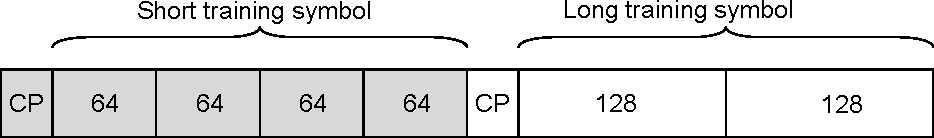
\includegraphics [width=0.7\columnwidth] {figures/Preamble.pdf} }
	\caption{Downlink preamble symbols for IEEE802.16.}
	\label{fig:pre}
\end{figure}

\begin{figure}
	\centerline{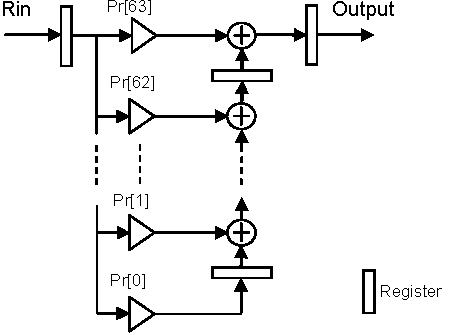
\includegraphics [width=0.5\columnwidth] {figures/structure_correlator.pdf} }
	\caption{Transpose Direct Form of Correlator.}
	\label{fig:str_corr}
\end{figure}


The 64 samples in the short symbol are used to perform cross-correlation with received samples for timing synchronisation. 
Therefore, the correlators are designed to compute cross-correlation with 64 constant coefficients. 
In this chapter, we explore two approaches to implementing such correlators. 
The first is based on Xilinx Virtex-6 FPGA DSP48E1 Slices, the standard approach to such an implementation.
The second is using multiplierless correlation implemented on both a Xilinx Virtex-6 and a low power Xilinx Spartan-6 device.
Both are designed to receive real and imaginary 16-bit samples in Q1.15 fixed point format. 
The output is the sum of 64 coefficient products, each being smaller than unity. 
So, the complex output words are in 21-bit fixed point Q6.15 format. 

If such a design was implemented blindly, with no consideration for the FPGA architecture, the synthesis tools would infer the use of embedded DSP blocks for multiplication, but would likely achieve poor timing due to an inability to optimise the use of the DSP block.
The DSP48E1 primitives on the Virtex-6 FPGAs have additional circuitry within them that enables the design of optimised datapaths, but this must be done manually, through writing code in a particular style.
Otherwise, the synthesis tools cannot always infer the most efficient structure.
In our design, we have taken into account the internal structure of the DSP block, and made the design as lean as possible.
The multiplierless design is specified entirely manually, and thus cannot be inferred by the tools.

%---------------------------------------------------------------------------------
\subsection{Design of DSP48E1 Based Correlator}

The DSP48E1 Slice inside the Virtex-6 shown in Fig. \ref{fig:DSP48E1} contains a multiplier followed by a configurable arithmetic unit to provide many independent functions, e.g., multiply, multiply accumulate, multiply add, three-input add, and more \cite{Xilinx2011}.
It also allows the datapath to be configured for various imput combinations and register stages; a three-stage pipeline offers maximum performance.
Since the DSP Slice is designed to mirror the structure of an FIR filter tap, it is ideally suited to implement correlation, and would hence be the method of choice for this application. 
Our first design uses non-pipelined DSP48E1 Slices in transpose direct form, as shown in Fig. \ref{fig:str_corr}, with 64 coefficients corresponding to the 64 samples in the preamble. 
The coefficients are pre-computed according to the IEEE802.16d standard. 
The second design spreads the complex multiply-adds in a five-stage pipeline, shown in Fig. \ref{fig:Cmp_MultAdder}, consisting of DSP48E1 Slices configured for three stage internal pipelining.  
$Ri\_Re$, $Ri\_Im$ are the real and imaginary parts of received sample, respectively. 
$Pr\_Re$, $Pr\_Im$ similarly represent known preamble. 
The pipeline registers for the $Pr\_Re$, $Pr\_Im$ are eliminated because they are considered to be of constant value. 
$Re$, $Im$ are the real and imaginary parts of the previous multiply-add. 
Fig. \ref{fig:DSP48pp_correlator} presents the pipeline structure of the correlator. 
The additional pipeline registers are required for handling the received sample.
Adding pipeline registers should increase performance significantly.
\begin{figure}
	\centerline{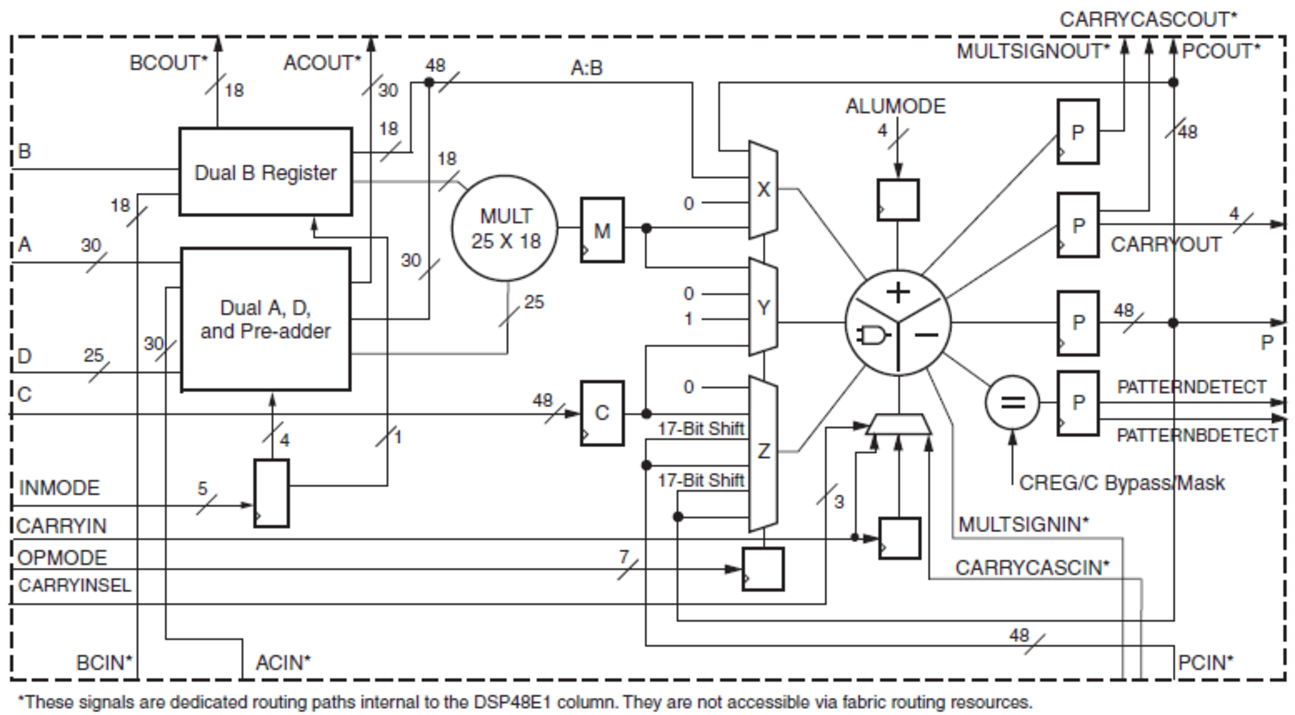
\includegraphics [width=0.9\columnwidth] {figures/DSP48E1.pdf} }
	\caption{Structure of DSP48E1 slice inside the Virtex-6 \cite{Xilinx2011}}
	\label{fig:DSP48E1}
\end{figure}

\begin{figure}
	\centerline{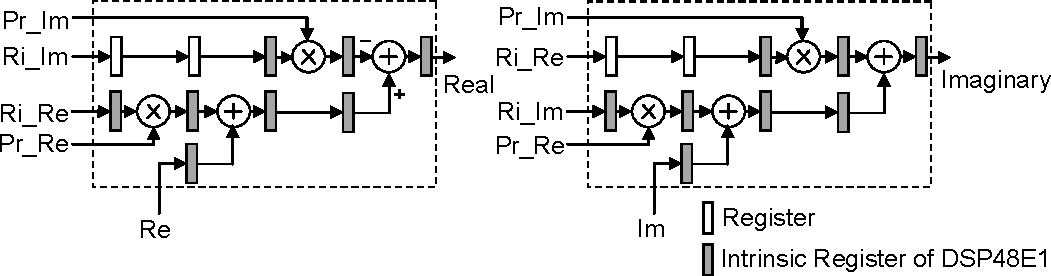
\includegraphics [width=0.9\columnwidth] {figures/Cmp_MultAdder.pdf} }
	\caption{Pipeline structure of the complex number multiply-add.}
	\label{fig:Cmp_MultAdder}
\end{figure}

\begin{figure}
	\centerline{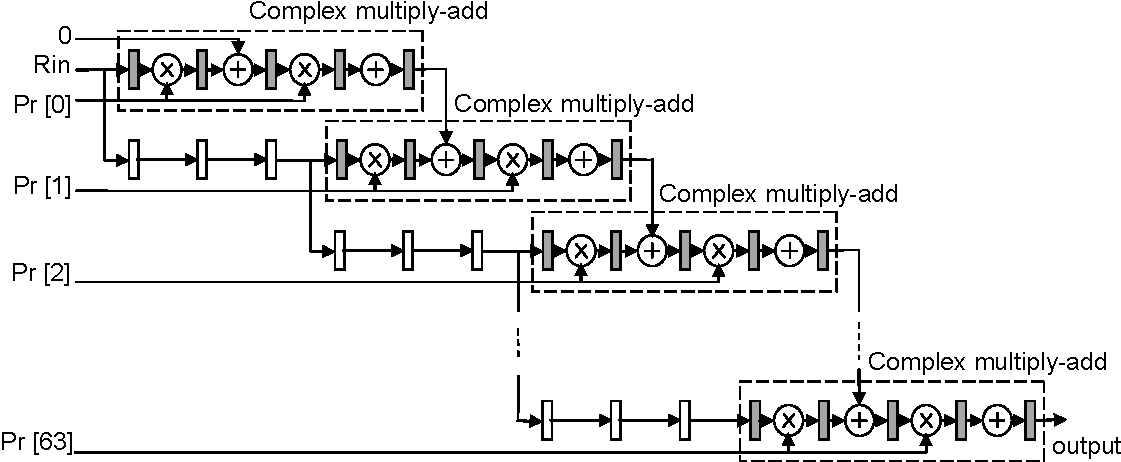
\includegraphics [width=0.9\columnwidth] {figures/DSP48pp_correlator.pdf} }
	\caption{Pipeline structure of correlator using DSP48E1 Slices.}
	\label{fig:DSP48pp_correlator}
\end{figure}

\begin{figure}
	\centerline{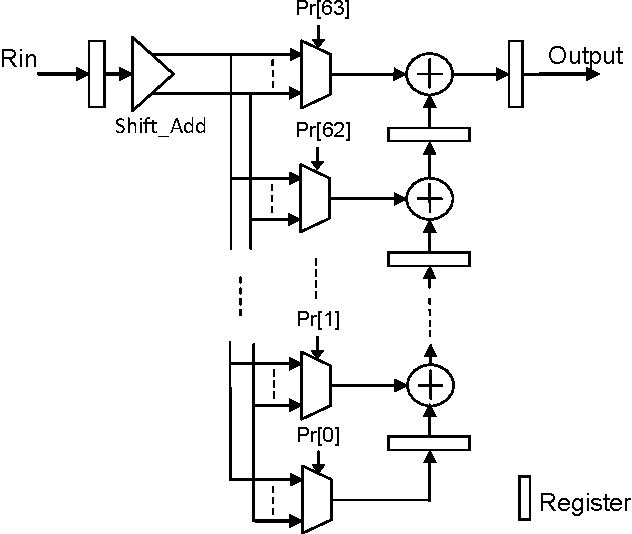
\includegraphics [width=0.7\columnwidth] {figures/ML_correlator.pdf} }
	\caption{Structure of multiplierless correlators.}
	\label{fig:ML_correlator}
\end{figure}

%---------------------------------------------------------------------------------
\subsection{Design of Multiplierless Correlator}

The principle of multiplierless correlators is to represent the coefficients and round them in the form of summed powers of two. 
Hence, a shift and add are performed instead of multiplying by coefficients. 
It is expected that multiplierless correlation is more efficient, but with embedded hard multipliers in modern FPGAs, it is unclear whether they should still be considered favourable. 
Furthermore, synchronisation accuracy must be considered.
To explore this, four alternative multiplierless correlators are implemented using four coefficient sets with an increasing degree of rounding, to compare the cost and performance and evaluate against multiplier-based correlators. 
The coefficient sets are found by quantising the 64 normalised preamble samples with quantisations of 1, 0.5, 0.25, and 0.125. 

The proposed structure for multiplierless correlators is shown in Fig. \ref{fig:ML_correlator}. 
This structure is based on the transpose-direct-form in Fig. \ref{fig:str_corr}. 
Instead of using multipliers to multiply input samples by coefficients, the $Shift\_Add$ block and multiplexers are used to perform the equivalent operation without an actual multiplication. 
But the  $Shift\_Add$ block, multilexers and value of $Pr[n]$ are different depending upon the quantised coefficient set being used.  
The $Shift\_Add$ block performs shift and add on received samples according to the degree of quantisation that is applied.  
To optimise resources in the case of small numbers of bit quantisation, one common $Shift\_Add$ block is used for all 64 coefficients instead of 64 separate $Shift\_Add$ blocks. 
This common $Shift\_Add$ block calculates all possible values for 64 coefficients.  
The multiplexers are used to select the corresponding values from $Shift\_Add$ to accumulate in order to generate the correlator output.
These are based on expressed coefficients $Pr[n]$ that are pre-computed based on quantizing the 64 preamble samples.
Since the $Pr[n]$ values are constants, after synthesising the design, the multiplexer is optimised as hard-wired logic, and the preamble cannot be changed.
To support different OFDM preambles, the $Pr[n]$ could be stored in a register, and a real multiplexer used instead of hard-wired logic.  
This results in increased resource utilisation but provides a more flexible solution. 

\subsection{Implementation Results}

The designs presented were synthesised and fully implemented using Xilinx ISE 13.2, targetting Xilinx Virtex-6 (V6) and Spartan-6 (S6) devices.  
The results of implementation are reported in terms of the number of occupied slices, DSP48E1s Slices and maximum frequency as summarised in Table \ref{tab:Imp_Rpt}. 

% Virtex-6 75T & Spartan-6 75T
\begin{table}[h]
	\centering
	\caption{Implementation Report}
	\label{tab:Imp_Rpt}
	\begin{tabular}{c|r|r|r|c|c}
        \hline \hline
    			Design  & \multicolumn{2}{|c|}{Occupied Slices} & DSP48E1s & \multicolumn{2}{|c}{Freq. (MHz)} \\
	\cline{2-6}			         & \makebox[1.2cm][c]{V6} & \makebox[1.2cm][c]{S6}& 	\makebox[1.2cm][c]{V6}	&  V6 & S6    \\
    	\hline
			DSPc 	& 742 		(6\%)  & -  			 & 256 (88\%) & 119 & -\\
			DSP\_pp &  1,110 	(9\%) & -  			 &  256 (88\%)& 398 & -\\
 			ML1 	&  661		(5\%) &	762 (6\%)	 &  0 (0\%)	& 309 & 174\\
			ML2 	&  983 	(8\%) &	1,071 (9\%) &  0 (0\%)	& 268 & 158\\
			ML3 	&  1,191 	(10\%) &	1,257 (10\%) &  0 (0\%)	& 234 & 136\\
			ML4 	&  1,496 	(12\%) &	1,517 (13\%) &  0 (0\%)	& 208 & 124\\   
    
    	\hline \hline  
    \end{tabular}	
\end{table}

$DSPc$, $DSP\_pp$ are correlator designs using DSP Slices, in non-pipelined and pipelined structures, respectively. 
$ML1$, $ML2$, $ML3$, $ML4$ are multiplierless correlators with coefficient quantisations of 1, 0.5, 0.25, 0.125, respectively.

Table \ref{tab:Imp_Rpt} reveals that the $DSP\_pp$ uses more logic slices due to its pipeline structure. 
The slices in DSP48E1 based designs are used for registers and route-thrus while the slices in the multiplierless designs are mostly used as logic. 
The number of slices used in the multiplierless designs increases as the coefficient quantisation becomes finer. 
The DSP48E1-based designs use 256 DSP Slices, 4 for each complex multiply plus 6-9\% of logic resources.
The multiplierless designs use only logic to compute the cross correlation with 64 complex coefficients. 
The total logic area is a small fraction of the whole device: around 5-12\% of total resources in the Virtex-6, and around 6-13\% of total resources in the equivalent Spartan-6.
While Spartan-6 devices do include DSP Slices, their number is insufficient to implement the full 64 sample complex cross correlation.
This shows an ideal scenario where multiplierless correlation makes sense, and hence serves as a motivation for this study.

The maximum frequencies, reported after place and route, decrease for multiplierless designs according to the degree of coefficient quantisation. 
Meanwhile the non-pipelined DSP48E1 design is slower than the multiplierless designs. 
However, the pipelined DSP48E1 design can achieve higher frequency.

A post-place-and-route simulation in ModelSim was used to estimate the power consumption of the system using the Xilinx XPower tool. 
Table \ref{tab:PWR} shows the power dissipation of the designs running at 50{\thinspace}MHz. 
The DSP48E1-based correlators consume more power than the multiplierless correlators, but this is due primarily to increased dynamic power when using the DSP48E1s on the Virtex-6. 
The dynamic power of the non-pipelined DSP48E1-based correlator $DSP\_Cor$ is greatest at 846{\thinspace}mW, but pipelining reduces this by a factor of more than 2.5 times, due to reduced switching activity between the multiplier and adder.  
The dynamic power of the multiplierless designs increases from 133{\thinspace}mW to 203{\thinspace}mW on Virtex-6 and from 149{\thinspace}mW to 294{\thinspace}mW on Spartan-6 as finer coefficient quantisation is used. 
It is important to note that the quiescent power of the Spartan-6 is much lower by design. 
Hence, we can see that using this multiplierless technique allows us to implement synchronisation on a Spartan-6 device, where a multiplier-based design is not possible, saving significant power and sacrificing little in terms of accuracy.

 % Virtex-6 75T  &  Spartan-6 75T
\begin{table}[h]
	\centering
	\caption{Power Consumption at 50MHz.}
	\label{tab:PWR}
	\begin{tabular}{c|c|c|c|c|c|c}
        \hline \hline
    			Correlators  & \multicolumn{2}{|c|}{Quiescent(mW)} &  \multicolumn{2}{|c|}{Dynamic(mW) }& \multicolumn{2}{|c}{Total(mW)} \\
	\cline{2-7}			& V-6 & S-6 & V-6 & S-6 & V-6 & S-6\\
	\hline
			DSP\_Cor		&  1312 &  -  	 & 846 & -	& 2158 &-\\
			DSP\_pp\_Cor 	& 1300  &  -   & 328 & - 	& 1628 & -\\
 			ML1\_Cor 		& 1296  & 67 & 133 & 149	& 1429 & 216\\
			ML2\_Cor 		& 1296  & 68 & 160 & 197	& 1456 & 265\\	
			ML3\_Cor 		& 1297  & 70 & 182 & 239	& 1479 & 309\\
			ML4\_Cor 		& 1297  & 71 & 203 & 294    & 1500 & 365\\   
    
    	\hline \hline  
    \end{tabular}
\end{table}


\begin{figure}
	\centerline{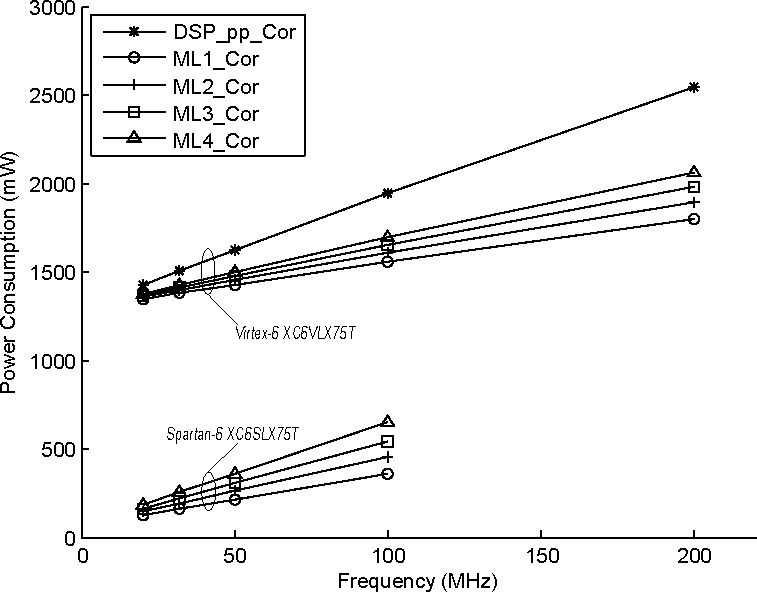
\includegraphics [width=0.9\columnwidth] {figures/Plot_PWR.pdf} }
	\caption{Power consumption of designs.}
	\label{fig:Plot_PWR}
\end{figure}

We also investigated how total power consumption varies with frequency, as shown in Fig. \ref{fig:Plot_PWR}.
As frequency increases, the finer quantisations and DSP48E1-based designs begin to consume proportionally more power.
Overall, multiplierless designs on the Spartan-6 consume 75\% to 85\% less power than the same designs on the Virtex-6, and a 0.25 quantisation design on the Spartan-6 consumes 81\% to 85\% less power then the DSP48E1-based design on a Virtex-6.

The \emph{DPS\_Cor} implementation represents how a ``blind'' design would be mapped. Our architecture-aware designs show significantly better performance, reduced area, and reduced power consumption.

%---------------------------------------------------------------------------------
\section{Simulation and discussion}
%---------------------------------------------------------------------------------
In order to validate our designs at the application level, we simulate them using ModelSim with an IEEE802.16 OFDM frame created using MATLAB, including the preamble symbols, data symbols and effects of an AWGN channel. 
Cross-correlation results using the correlator designs are compared to corresponding results in MATLAB to verify the correctness of implementation. 
To evaluate the accuracy of timing synchronisation acheivable by these designs, the correlation outputs are plotted in Fig. \ref{fig:Plot_XCR} for random data frames at 10{\thinspace}dB SNR. 
The output of each correlator is slightly different because of rounding, but the timing synchronisation depends upon the location of the peaks being at the  position of the preamble.
All the correlator designs achieve this most of the time, as shown at indices 34 and 98 for the CP samples and the first preamble samples respectively, for a single frame. 
 
\begin{figure}
	\centerline{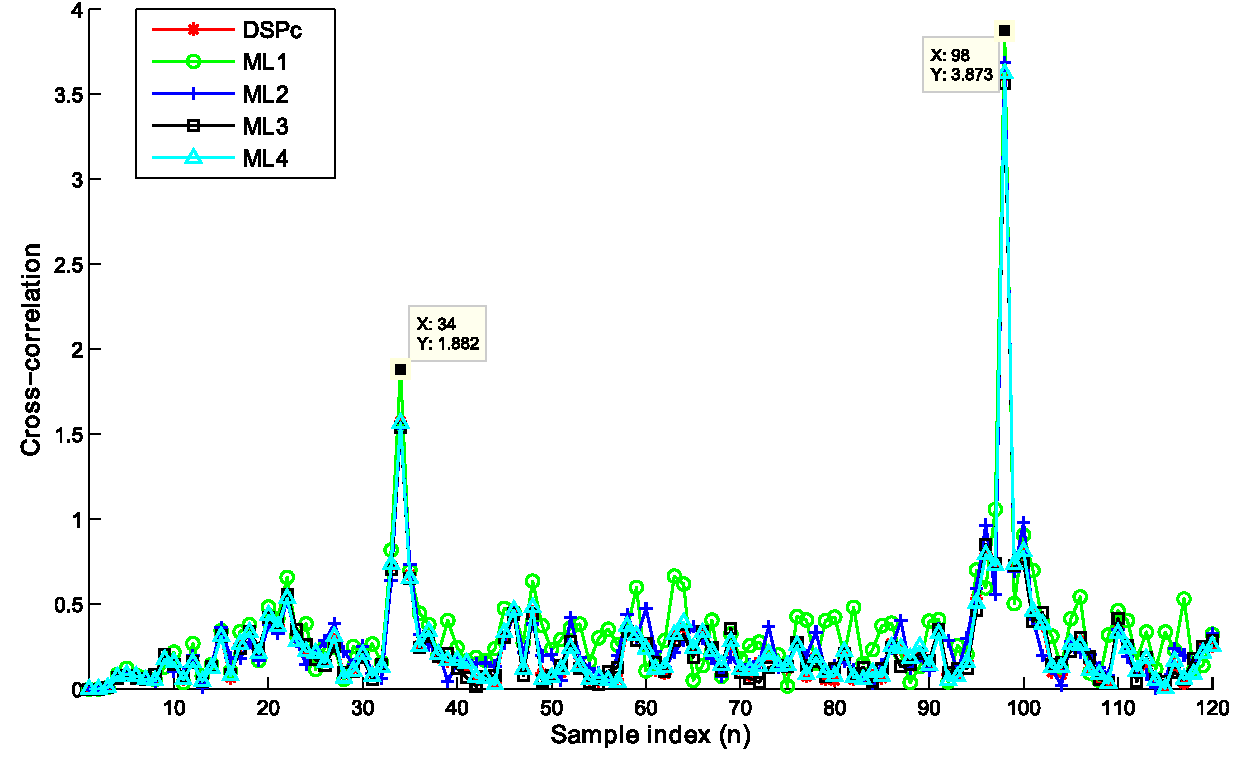
\includegraphics [width=0.9\columnwidth] {figures/Plot_XCR.pdf} }
	\caption{Correlator output with SNR = 10dB.}
	\label{fig:Plot_XCR}
\end{figure}

In order to evaluate the synchronisation accuracy of these approaches, we simulate 10,000 correlation operations in an AWGN channel with a detection strategy as follows. 
First, find the first peak, $P1$, over 64 samples. 
Next, find the second peak, $P2$, in the next 64 samples from the first peak and compute average value, $avg$, of the samples between two peaks. 
If  $( P1 - avg ) \le  0.75 * ( P2 - avg )$, the start of frame is detected and the correctness of the position can be checked. 
It should be noted that in all cases, the peaks were known to be located within the two search regions and that the detection strategies described above are compatible with those of other authors such as \cite{Kishore2006} and \cite{Yip2003}. 
Fig. \ref{fig:Plot_NFail} plots the results in terms of failure rate against AWGN SNR and show that the designs are able to accurately detect the start of frame even in low SNR conditions. 
The failure rate of $ML1\_Cor$ is the highest, as expected, due to the coarse quantisation.
For SNRs above 4{\thinspace}dB, the failure rates of $ML2\_Cor$, $ML3\_Cor$,  $ML4\_Cor$ and $DSP\_Cor$ differ less than 0.05\% from each other.
This suggests that sacrificing accuracy by using multiplierless cross-correlation is feasible and has negligible impact on synchronisation accuracy.
Combined with the results in the previous section, we can be confident that low-power FPGAs, such as the Spartan-6, with insufficient resources for multiplier-based synchronisation correlation, are still feasible for implementing robust OFDM receivers.

\begin{figure}
	\centerline{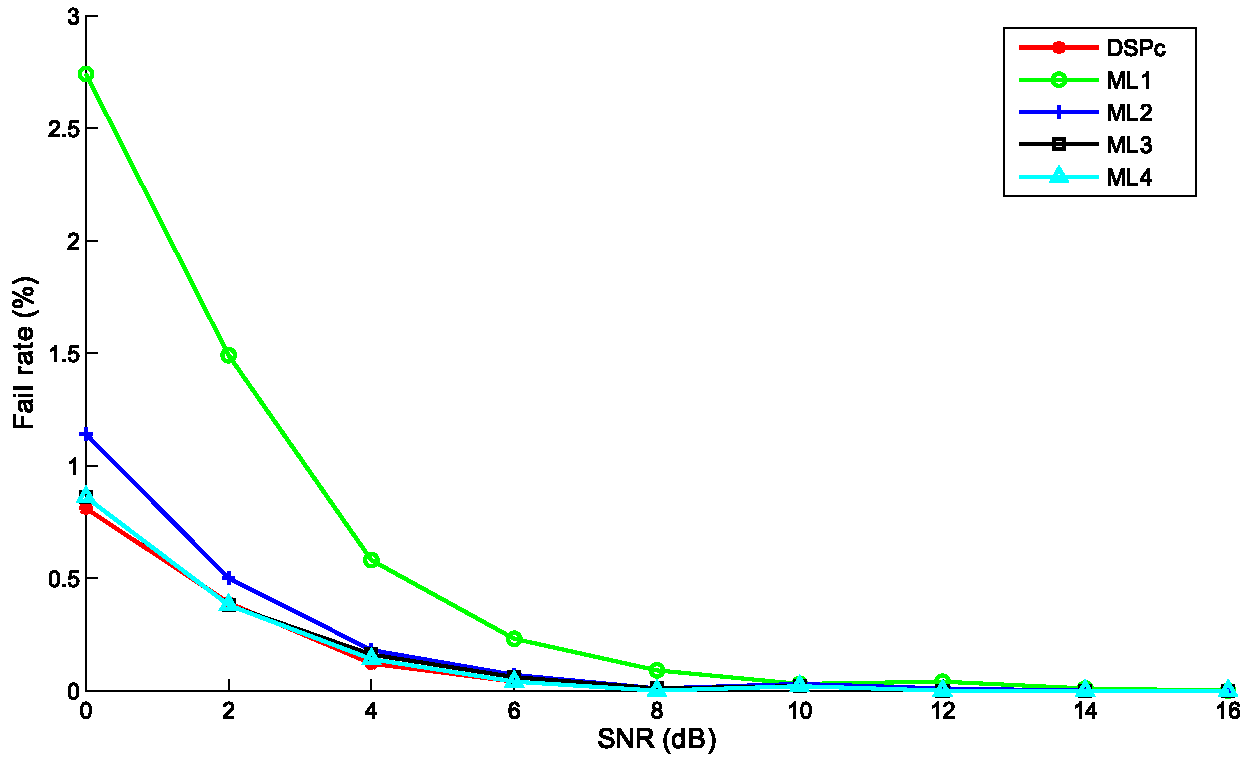
\includegraphics [width=0.85\columnwidth] {figures/Plot_NFail.pdf} }
	\caption{Detection failure rate.}
	\label{fig:Plot_NFail}
\end{figure}

%---------------------------------------------------------------------------------
\section{Summary}
%---------------------------------------------------------------------------------
The DSP48E1 Slices on modern Virtex-6 FPGA devices seem to offer the ideal resource for implementing correlation-based frame synchronisers.
However, as we have discovered, in the context of synchronisation for IEEE802.16 OFDM systems, simplified multiplierless designs offer comparable synchornisation performance. 
While the DSP48E1-based correlators can obtain higher clock speeds, this is only possible through a detailed pipelined design.
Furthermore, their power consumption and resource usage is considerably greater.
Since low-power, low-cost devices such as the Xilinx Spartan-6 do not include sufficient DSP Slices, this suggests adopting multiplierless designs for low-power implementations.
We have shown that while very low quantisation resolution does impact synchronisation performance, with a step size of just 0.5, synchronisation accuracy is on par with multiplier-based correlation. 
Multiplierless correlation on a Spartan-6 can save over 85\% power compared to  a DSP Slice design on a Virtex-6 FPGA.

This work has been submitted as a journal paper to  IEEE transactions on Very Large Scale Integration (VLSI) systems.